\documentclass[a4page]{article}

\usepackage{graphicx}
\usepackage{textpos}
\usepackage{hyperref}
\usepackage{xcolor}
\usepackage{enumitem}

\setitemize[1]{leftmargin=0ex,labelsep=10pt}

\newcommand\hsep{ {\color{gray}/} }
\newcommand\partitle[1]{\vskip20pt\par\noindent{\textsf{\textbf{#1}}}}

\usepackage{fontawesome}

\begin{document}

\begin{textblock}{2}(7,-.7)
    \noindent
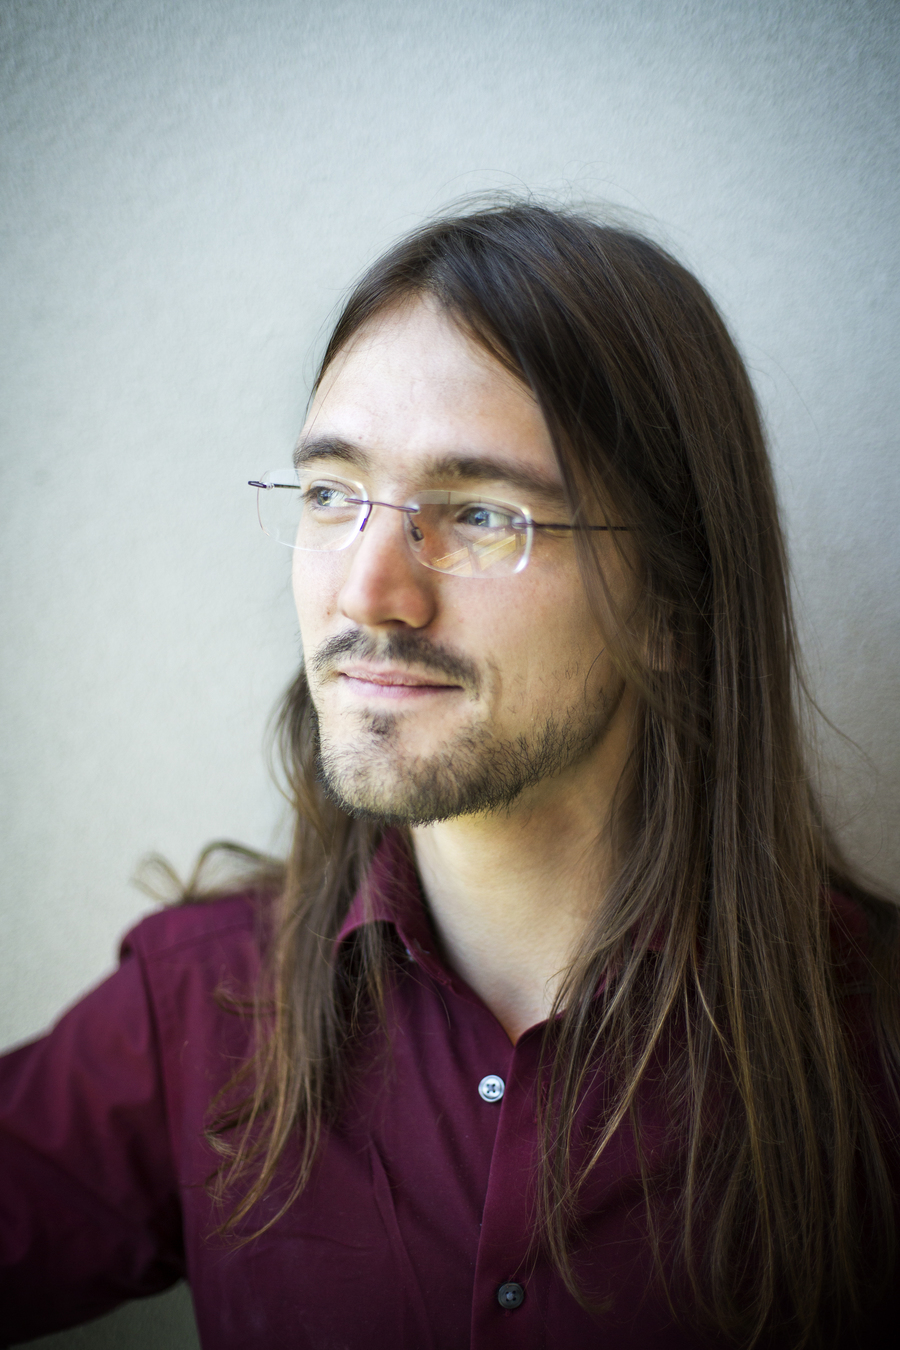
\includegraphics[width=\textwidth]{me}
        \footnotesize(2019)
\end{textblock}\noindent
\textsf{\Large dr.~Bas Westerbaan}\\
engineering curriculum vitae Januari~2021\\

\noindent
\href{mailto:bas@westerbaan.name}{\faEnvelopeO\ bas@westerbaan.name} \hsep
\href{https://bas.westerbaan.name}{\faExternalLink\ bas.westerbaan.name}\\
\href{https://scholar.google.nl/citations?user=AN7BEa8AAAAJ}{%
    \faGraduationCap\ Google Scholar}
    \hsep \href{https://github.com/bwesterb}{\faGithub\ \texttt{bwesterb}}
    \hsep \href{https://www.linkedin.com/in/baswesterbaan/}{\faLinkedinSquare} \\
$*$ 1988, the Netherlands

\vskip0.3cm\noindent
I'm a mathematical software engineer: I combine a deep understanding
    of mathematics and computer architecture
    with the practical know-how to get things into production.
    I enjoy solving  problems that seem intractable
        with off-the-shelf solutions.

My doctoral research focussed on quantum computing.
In recent years I've become particularly interested
    in crytography engineering and have made world-class contributions
        (e.g.~as a cosubmitter of the
	\href{https://sphincs.org/data/sphincs+-round3-specification.pdf}{SPHINCS$^+$}
    signature scheme that is in round 3 of the NIST post-quantum competition.)

\partitle{Career}
\begin{itemize}
    \item[2020 --] \emph{Post-doctoral researcher} (crypto engineering) --- Radboud Universiteit\\
        At the Digital Security group under prof.~Schwabe,
            I continued the work started at Cloudflare, see below.
    \item[sept.~2020] \emph{Freelance developer} --- Stichting Privacy by Design\\
        I helped design, implement and deploy \href{https://qrona.info}{qrona.info}.
    \item[2019 -- 2020] \emph{Cryptography research fellow} (0.2fte) --- 
        \href{https://cloudflare.com}{Cloudflare} \\
        At the cryptography group of Nick Sullivan, I've
            worked on making TLS secure against quantum computers.
        This is a broad task that included:
                designing and performing large-scale measurements on network
                    performance;
                implementing new cryptographic primitives;
                designing changes to core protocols and
                    preparing internal infrastructure for these changes.
    \item[2019 -- 2020] \emph{Post-doctoral researcher} (1fte) --- University
        College London\\
        At the \href{http://pplv.cs.ucl.ac.uk/welcome/}{PPLV group}
            under \href{https://alexandrasilva.org/#/main.html}{prof.~dr.~Silva}.
    \item[2018 -- 2019] \emph{Cryptography engineer} --- Radboud Universiteit\\
        On the \href{https://pep.cs.ru.nl}{Polymorphic Encryption and Pseudonymisation (PEP) project}.
        Working with five colleagues, I made giant leaps in the practical usability
        of this data store at scale.

            
    \item[2013 -- 2018]  \emph{Promovendus (Ph.D-student) ---
        Radboud Universiteit}\\
        At the \href{http://www.ru.nl/ds/}{Digital Security group}
        of Radboud University funded by
        the ERC Advanced Grant \href{https://cordis.europa.eu/project/rcn/107285_en.html}{`Quantum Logic, Computation and Security'}
        of \href{http://www.cs.ru.nl/B.Jacobs/}{prof.~dr.~Bart Jacobs}.
            Defended
            \href{http://westerbaan.name/~bas/thesis.pdf}{thesis}
            on May 14th, 2019.
    \item[2007 -- 2013] \emph{B.Sc \& M.Sc degrees in Mathematics ---
                Radboud Universiteit} \\
        M.Sc thesis \href{www.ru.nl/publish/pages/813276/masterscriptie_bas_westerbaan.pdf}{`Sequential Product on Effect Logics'}
            supervised by \href{http://www.cs.ru.nl/B.Jacobs/}{prof.~dr.~Jacobs} \hsep
        B.Sc thesis \href{https://arxiv.org/abs/1409.1030}{`On Effective Undecidability and Post's Problem'}
            supervised by \href{http://www.ru.nl/wiskunde/@1039532/veldman-dhr-dr-(wim)/}{dr.~Veldman}.
        The Master's degree was awarded \emph{cum laude}.
    \item[2006 -- 2007] \emph{Freelance developer} (part-time)
        for software licensing database used by Dutch police.
\end{itemize}

\partitle{Relevant experience}
\begin{itemize}
    \item Performed influential \textbf{security audits} (whole spectrum:
        blackbox, pentest, reverse
        engineering, code review, reporting, advise)
        on apps for DigiD (Dutch government identity system);
        Belastingdienst (Dutch IRS) 
        and Osiris (Dutch student grade registration)
        supervised by prof.~dr.~Marko van Eekelen,
        2016--2017.
    \item \href{https://github.com/bwesterb}{Various contributions} to the open source community, among others:
        \begin{enumerate}
            \item \href{https://github.com/bwesterb/go-xmssmt}{\texttt{go-xmssmt}}, Go implementation of the XMSS\textsuperscript{MT}
                        signature scheme.
                \item Helped out with
        \href{https://github.com/signalapp/curve25519-dalek/commit/c2320e9137ab1d02234620ed4f3b22371f688db2}{Ristretto
                    group encoding} for the \href{https://signal.org/en/}{Signal} private messenger.
            \item \href{https://github.com/cloudflare/circl}{\texttt{circl}}, Go implementation of
                    Kyber and Dilithium.
            \item \href{https://github.com/sphincs/sphincsplus}{\texttt{sphincsplus}},
                    speed improvements to SPHINCS$^+$ signature scheme reference and optimized implementations.
            \item \href{https://github.com/bwesterb/py-seccure}{\texttt{py-seccure}}, Python implementation of SECCURE elliptic curve toolkit.
            \item \href{https://github.com/bwesterb/py-tarjan}{\texttt{py-tarjan}}, Python implementation of Tarjan's algorithm.
            \item \href{https://github.com/bwesterb/pol}{\texttt{pol}}, password manager with deniable encryption.
            \item \href{https://github.com/msgpack/msgpack-python/pull/42}{Pure Python fallback of \texttt{msgpack}}, a popular data interchange format.
            \item \href{https://github.com/bwesterb/go-ristretto}{\texttt{go-ristretto}}, Go implementation of the Ristretto prime-order group.
            \item \href{https://github.com/bwesterb/argon2pure}{\texttt{argon2pure}}, Python implementation of the Argon2 hash and its inclusion
                    in Django.
        \end{enumerate}
    \item I have ten years of experience as a \textbf{teaching assistant}
            and have \textbf{lectured} a course on computer networking
            at the Radboud University.
    \item Member \textbf{student board} science faculty Radboud Universiteit
        2011 -- 2012.
    \item \textbf{Secretary of the board} of the 150-member student
        club Karpe Noktem 2010--2011.
        I've also led their IT group ($\sim$5 people)  2008--2018.
\end{itemize}

\partitle{Breadth}\\
I am a quick learner\footnote{%
    For instance, the first time I wrote assembly was on the job
    at Cloudflare, where I quickly improved world-record performance numbers
    (for fourway SHA3.)}
--- nonetheless I'll list some languages, frameworks
  and other technologies I have previous experience with:
C, Python, Assembler (AVX2, NEON), Go, C++, Linux, macOS, git, svn,
    Rust, Java, Javascript, LaTeX, Haskell, C\textsuperscript{\#},
    Ruby, Django, webassembly, R, numpy, scipy, coq, kubernetes,
    cuda, PHP, mysql, postgres, mongodb, ansible, grafana, prometheus,
    nginx, bind, intrinsics.

\partitle{Academic career}\\
See my \href{https://westerbaan.name/~bas/cv.pdf}{academic curriculum vitae}
    for a list of publications and other academic achievements.

\partitle{Personal}\\
I enjoy gourmet cooking and bouldering.
\end{document}

% vim: ft=tex.latex
